\documentclass[main.tex]{subfiles}
% 线性算符的行列式、迹、特征值分解
\begin{document}
线性算符的行列式、迹和特征值,都是关于一个线性算符的标量,而且这些标量的取值不依赖基的选择。
%========================================================
\subsubsection{线性算符的行列式}
\begin{definition}[$n\times n$矩阵的行列式]\label{def:II.2.17}
    设$A$是数域$\mathbb{F}$上的$n\times n$矩阵(记为$A\in\mathbb{F}^{n\times n}$),$a_i=\left(A_{i1},\cdots,A_{in}\right),i=1,\cdots,n$是$A$的第$i$行的有序数组,如果函数$D:\mathbb{F}^{n\times n}\rightarrow\mathbb{F}$满足:
    \begin{enumerate}
        \item $D$是关于$\left(a_1,\cdots,a_n\right)$的$n$重线线性函数,即
              \[
                  D\left(a_1,\cdots,\lambda a_i+a^\prime_i,\cdots,a_n\right)=\lambda D\left(a_1,\cdots,a_i,\cdots,a_n\right)+D\left(a_1,\cdots,a^\prime_i,\cdots,a_n\right),\forall\lambda\in\mathbb{F}
              \]
        \item 当$A$的任意两行相等则$D\left(A\right)=0$
        \item 设$A^\prime$是$A$的任意两行调换后的矩阵,则$D\left(A^\prime\right)=-D\left(A\right)$
        \item $D\left(I\right)=1$,其中$I$是$n\times n$单位矩阵
    \end{enumerate}
    则称$D$是\emph{矩阵$A$的行列式(determinant)},记为$\mathrm{det}A$。
\end{definition}
上述定义中的条件1是本身是\emph{$n$重线性函数($n$-linear function)}的定义,条件1和条件2一起则是\emph{交替(alternating)}$n$重线性函数的定义。条件3是可由条件1和2独立证明得到的(此略\cite[\S 5.2]{Hoffman1971}),加到了定义中只是为了便于理解。我们可以说,行列式就是一个关于$n\times n$矩阵的交替$n$重线性标量值函数且附加满足条件4。

上面的定义隐含默认了任意一个$n\times n$矩阵的行列式是唯一存在的要求(因为“函数”的定义本身要求这一条),但这未被证明。本讲义暂不列出详细证明的证明过程,只简述证明的思路。证明存在性往往相当于于找到这一存在。回顾本科的线性代数课本,我们发现那里的定义方式\cite[\S 1.3 定义3.1]{周胜林2012线性代数}就帮我们找出了这一存在:
\[
    \mathrm{det}A=\sum_{\sigma}\left(\mathrm{sgn}\sigma\right)A\left(1,\sigma_1\right)\cdots A\left(n,\sigma_n\right)
\]
其中$A\left(i,j\right)\equiv A_{ij}$;$\sigma_i,i=1,\cdots,n$表示$n$阶排列$\sigma$的一种;$\mathrm{sgn}\sigma$是根据$\sigma$的奇偶性取值1或$-1$\footnote{关于$n$阶排列的知识可参见\cite[\S1.2]{周胜林2012线性代数}。}。作为存在性的证明,提出这一公式,然后验证其满足行列式定义中的条件,就完成了。而唯一性的证明则需要如下引理:任意$\mathbb{F}^{n\times n}$上的交替$n$重线性函数$D$均满足$D\left(A\right)=\mathrm{det}AD\left(I\right),\forall A\in\mathbb{F}^{n\times n}$,其中$\mathrm{det}A$在此只需存在即可。该引理的证明也可以从上述的行列式公式直接得出,使得行列式定义中的条件4实际成为行列式唯一性的必要条件。

以下定理列出了$n\times n$矩阵的行列式的一些性质,在本讲义中也不作证明而直接承认其成立,因为它们都已经大学一年级的线性代数课程中介绍过了。

\begin{theorem}\label{thm:II.2.24}
    \quad
    \begin{itemize}
        \item $\mathrm{det}\left(AB\right)=\mathrm{det}A\mathrm{det}B,\forall A,B\in\mathbb{F}^{n\times n}$
        \item $\mathrm{det}\left(A^\intercal\right)=\mathrm{det}A,\forall A,B\in\mathbb{F}^{n\times n}$
        \item ${A}$可逆$\Leftrightarrow\mathrm{det}\left(A\right)\neq 0$
        \item $\mathrm{det}\left(A^{-1}\right)=\left(\mathrm{det}A\right)^{-1},\forall A,B\in\mathbb{F}^{n\times n}$
        \item 如果$B$是$A$的第$i$行加上第$j$行的倍数得到的矩阵,则$\mathrm{det}B=\mathrm{det}A$

        \item \emph{克拉默法则(Cramer's rule)}\cite[\S1.5]{周胜林2012线性代数}
    \end{itemize}
\end{theorem}

定义在数域$\mathbb{F}$上的有限维向量空间$\mathcal{V}$上的线性算符$\mathbf{T}\in\mathcal{L}\left(\mathcal{V}\right)$在不同有序基下的坐标矩阵之间有变换公式。设$B,B^\prime$是$\mathcal{V}$的两组有序基,$S$是从$B$到$B^\prime$的过渡矩阵,则由定理\ref{thm:II.2.22}有$\left(\mathbf{T}\right)=S\left(\mathbf{T}\right)^\prime S^{-1}$,其中$\left(\mathbf{T}\right),\left(\mathbf{T}\right)^\prime$分别是$\mathbf{T}$在$B,B^\prime$下的坐标矩阵。由行列式的性质有$\mathrm{det}\left(\mathbf{T}\right)=\mathrm{det}\left[S\left(\mathbf{T}\right)S^{-1}\right]=\mathrm{det}\left(\mathbf{T}\right)^\prime$,因此\emph{一个线性算符在任意基下的坐标矩阵的行列式都相等}。由此我们可以直接定义“线性算符的行列式”,记为$\mathrm{det}\mathbf{T}$,为其在任一基下的坐标矩阵的行列式。正式定义如下。

\begin{definition}[线性算符的行列式]\label{def:II.2.18}
    设$\mathbf{T}$是$n$维向量空间$\mathcal{V}$上的线性算符,$B$是$\mathcal{V}$的一组有序基,则$\mathbf{T}$的行列式$\mathrm{det}\mathbf{T}\equiv\mathrm{det}\left(\mathbf{T}\right)$,其中$\left(\mathbf{T}\right)$是$\mathbf{T}$在$B$下的坐标矩阵。
\end{definition}
%===========================================================
\subsubsection{线性算符的迹}
从线性算符的行列式的定义过程,我们发现,与本科线性代数课上直接定义成一个运算公式不同,我们总是先定义一组代数规则,再去证明这样的代数规则唯一对应一个具体的运算公式。线性算符的迹也可按类似的方式重新定义。不过,既然已经通过行列式的例子来了解这种思想,此处关于迹的定义仍采用简化的方式。值得注意的是,迹是定义在\emph{内积空间}上的线性算符上的。

\begin{definition}[线性算符的迹]\label{def:II.2.19}
    设$\mathbf{A}$是数域$\mathbb{F}$上的内积空间$\mathcal{V}$上的线性算符,则$\mathbf{A}$的\emph{迹(trace)}为$\mathrm{tr}\mathbf{A}\equiv\sum_k\left(\mathbf{A}\mathbf{\hat{e}}_k|\mathbf{\hat{e}}_k\right)$,其中$\left\{\mathbf{\hat{e}}_k\right\}$是$\mathcal{V}$的任意一组规范正交基。
\end{definition}

易验,上述定义的迹的值不依赖基的选择而改变,从而任一线性算符唯一对应一个迹。我们还能进一步获得如下性质。

\begin{theorem}\label{thm:II.2.25}
    设$\mathbf{A}$、$\mathbf{B}$是数域$\mathbb{F}$上的内积空间$\mathcal{V}$上的任意两个线性算符,则
    \begin{enumerate}
        \item $\mathrm{tr}\left(\alpha\mathbf{A}+\mathbf{B}\right)=\alpha\mathrm{tr}\mathbf{A}+\mathrm{tr}\mathbf{B}$
        \item $\mathrm{tr}\left(\mathbf{AB}\right)=\mathrm{tr}\left(\mathbf{BA}\right)$
    \end{enumerate}
\end{theorem}

我们在此还可通过迹来定义$\mathcal{L}\left(\mathcal{V}\right)$空间上的一种内积。

\begin{definition}[线性算符的标准内积]\label{def:II.2.20}
    设$\mathbf{A},\mathbf{B}$是数域$\mathbb{F}$上的内积空间$\mathcal{V}$上的任意两个线性算符,令$\left(\mathbf{A}|\mathbf{B}\right)\equiv\mathrm{tr}\left(\mathbf{A}^*\mathbf{B}\right)$,可验证,该定义满足内积规定,称为线性算符的\emph{标准内积(standard inner product)},经常记作$\mathbf{A}:\mathbf{B}$。
\end{definition}

读者可尝试自行推导两个线性算符的标准内积在给定基下的坐标运算公式。
%======================================================================
\subsubsection{线性算符的特征值}
我们已经知道,向量空间上的线性算符在选定某组基下,它的性质就全由其坐标矩阵决定。线性算符的特征值分析,其实是对一个线性算符的“内部结构”像对钟表那般进行解剖,搞清楚它的运作方式。

尽管线性算符的特征值分析能给出很丰富的结论,但目前我们也许可以先从这样一种动机去引入线性算符的特征值定义。比如我们关心一个线性算符是否可逆,从线性变换的维数定理的角度,需要知道线性算符的秩,即其在任一选定基下的坐标矩阵的秩。从定理\ref{thm:II.2.24}的角度,需要知道线性算符的行列式,即其在任一选定基下的坐标矩阵的行列式。如果一个数域$\mathbb{F}$上的$n$维向量空间$\mathcal{V}$上的线性算符$\mathbf{T}$在基$\left\{\mathbf{a}_i\right\}$下的坐标矩阵是对角矩阵,即
\[\left(\mathbf{T}\right)=\left(\begin{array}{ccc}\lambda_1&&\\&\ddots&\\&&\lambda_n\end{array}\right),\lambda_i\in\mathbb{F},i=1,\cdots,n\]
就称线性算符$\mathbf{T}$是\emph{可对角化的(diagonalizable)}。此时有
\[\mathbf{Ta}_i=\lambda_i \mathbf{a}_i,\quad i=1,\cdots,n\]
$\mathbf{T}$的值域就是由$\lambda_i\neq 0$对应的$\mathbf{a}_i$线性生成的,$\lambda_i\neq 0$的个数就是$\mathrm{rank}\mathbf{T}$,要想$\mathbf{T}$可逆,必须使得$\mathrm{rank}\mathbf{T}=n$(满秩),或由$\mathrm{det}\mathbf{T}=\prod_{i=1}^n\lambda_i\neq 0$要求$\left(\mathbf{T}\right)$的对角元素全不为零。总之矩阵$\mathbf{T}$的很多性质就能确定了。

为了这一目标,我们先讨论一般的形如$\mathbf{Ta}=\lambda\mathbf{a}$的情况。

\begin{definition}[特征值、特征向量、特征空间]\label{def:II.2.21}
    设$\mathcal{V}$是数域$\mathbb{F}$上的有限维向量空间,$\mathbf{T}\in\mathcal{L}\left(\mathcal{V}\right)$是一个线性算符。若存在$\mathbf{a}\neq\mathbf{0},\mathbf{a}\in\mathcal{V},\lambda\in\mathbb{F}$满足$\mathbf{Ta}=\lambda\mathbf{a}$,则称$\lambda$是$\mathbf{T}$的一个\emph{特征值(characteristic value)},$\mathbf{a}$是$\mathbf{T}$对应于特征值$\lambda$的一个\emph{特征向量(characteristic vector)}。$\mathbf{T}$关于同一特征值$\lambda$的所有不同的特征向量的集合称为$\mathbf{T}$的\emph{特征空间(characteristic space)}。
\end{definition}

\begin{figure}[htbp]
    \centering
    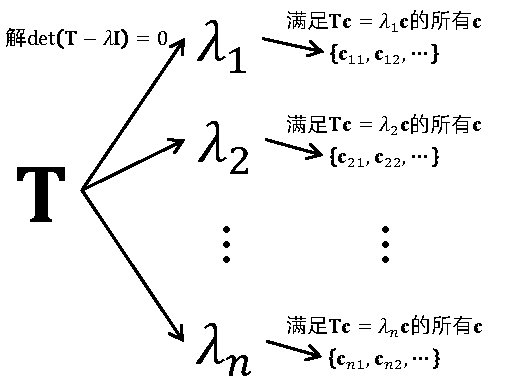
\includegraphics{images/characteristic_values.pdf}
    \caption{复数域上的$n$维向量空间上的线性算符$\mathbf{T}$有$n$个特征值,对应每个特征值都可能有一个或以上的特征向量。对应于每个特征值的所有特征向量的集合称为关于该特征值的特征空间。特征空间具有向量运算的封闭性(需证明),故它们都是所在向量空间的子空间。}
    \label{fig:II.2.3}
\end{figure}

由特征值和特征向量的定义可知,复数域上的$n$维向量空间上的线性算符可以有$n$个特征值。对应于同一个特征值,可能有多个特征向量。能够证明,关于同一特征值的特征空间是向量空间的一个子空间,作为定理如下。

\begin{theorem}\label{thm:II.2.26}
    设$\mathcal{V}$是数域$\mathbb{F}$上的有限维向量空间,$\mathbf{T}\in\mathcal{L}\left(\mathcal{V}\right)$是一个线性算符,则$\mathbf{T}$的特征空间是$\mathcal{V}$的子空间。
\end{theorem}
\begin{proof}
    设$\mathbf{a},\mathbf{b}\in\mathcal{V}$是关于$\mathbf{T}$的特征值$\lambda$的其中两个特征向量,则对任意$\alpha\in\mathbb{F}$有$\mathbf{T}\left(\alpha\mathbf{a}+\mathbf{b}\right)=\alpha\mathbf{Ta}+\mathbf{Tb}=\alpha\lambda\mathbf{a}+\lambda\mathbf{b}=\lambda\left(\alpha\mathbf{a}+\mathbf{b}\right)$。
\end{proof}

定义\ref{def:II.2.21}只告诉我们,如果有满足定义的东西,则把它称为什么;它没有告诉我们这样的东西存不存在,如何去求它们。为使特征值的概念更实用,我们进一步考虑一个重要的线性算符表达式。设$\mathcal{V}$是数域$\mathbb{F}$上的有限维向量空间,$\mathbf{T}\in\mathcal{L}\left(\mathcal{V}\right)$是一个线性算符,$\lambda$是$\mathbf{T}$的一个特征值,$\mathbf{a}$是$\mathbf{T}$关于$\lambda$的任一特征向量,则总有
\[\left(\mathbf{T}-\lambda\mathbf{I}\right)\mathbf{a}=\mathbf{Ta}-\lambda\mathbf{Ia}=\mathbf{0}\]
即$\mathbf{T}$关于$\lambda$的特征空间就是线性算符$\mathbf{T}-\lambda\mathbf{I}$的零空间。根据线性变换的维数定理,$\mathbf{T}$的特征空间的维数就是$\mathbf{T}-\lambda\mathbf{I}$的零化度,进而有如下定理。

\begin{theorem}\label{thm:II.2.27}
    设$\mathcal{V}$是数域$\mathbb{F}$上的有限维向量空间,$\mathbf{T}\in\mathcal{L}\left(\mathcal{V}\right)$是一个线性算符,则以下命题相互等价:
    \begin{enumerate}
        \item $\lambda$是$\mathbf{T}$的特征值
        \item $\mathbf{T}-\lambda\mathbf{I}$是奇异的
        \item $\mathrm{det}\left(\mathbf{T}-\lambda\mathbf{I}\right)=0$
    \end{enumerate}
    \begin{proof}
        我们在本科的线性代数课中已经了解,矩阵行列式为零,就是该矩阵相对就的一个线性方程组无非全零解,亦即该矩阵是不可逆的。这些结论的详细证明就是对$2\Leftrightarrow 3$的证明。此略。$1\Leftrightarrow 3$可利用行列式的性质简单证得,此略。
    \end{proof}
\end{theorem}

这一定理的第3个命题实际提供了一个求算给定线性算符的特征值的方法。因为
\[\mathrm{det}\left(\mathbf{T}-\lambda\mathbf{I}\right)\]
必是一个$\mathrm{dim}\mathcal{V}$阶首一多项式\footnote{这一命题的结论需要依靠多项式代数的知识来证明。后文还要用到代数基本定理,这个定理也是通过多项式代数证明的重要结论,此略\cite{Hoffman1971}。}。因此可将其定义为$\mathbf{T}$的\emph{特征多项式}\emph{(characteristic polynomial)},从而$\mathbf{T}$的任一特征值均为其特征多项式的一个根。在复数域上,由代数基本定理,$n$阶首一多项式有且必有$n$个复根(可能有重根)\footnote{这样的数域又叫代数闭域。例如实数域就不是代数闭域。所以线性算符所有关于特征值的性质,在实数域上都需要小心是否会丧失。}。因此我们可以说复数域上任一$n$维线性空间上的线性算符必有$n$个特征值;解其特征多项式就可以得到它们全部。

本节开头提出的,希望线性变换在某组基下的坐标矩阵是对角矩阵,这相当于要求线性变换的特征向量直接就是一组基。我们可以从这一要求出发,找出与其等价的一系列命题,如以下定理所示。

\begin{theorem}\label{thm:II.2.28}
    设$\mathcal{V}$是数域$\mathbb{F}$上的$n$维向量空间,$\mathbf{T}\in\mathcal{L}\left(\mathcal{V}\right)$是一个线性算符,$\left\{\theta_1,\cdots,\theta_k\right\}$是$\mathbf{T}$的两两不同的特征值,$\mathcal{W}_i$是线性算符$\mathbf{T}-\theta_i\mathbf{I}$的零空间,则以下命题相互等价:
    \begin{enumerate}
        \item $\mathbf{T}$是可对角化的;
        \item $\mathbf{T}$的特征多项式是
              \[\left(\theta-\theta_1\right)^{d_1}\cdots\left(\theta-\theta_k\right)^{d_k}\]
              且
              \[\mathrm{dim}\mathcal{W}_i=d_i,\quad i=1,\cdots,k\]
        \item $\mathrm{dim}\mathcal{V}=\sum_{i=1}^k\mathrm{dim}\mathcal{W}_i$
    \end{enumerate}
\end{theorem}

这一定理第1、2条之间的等价性可见\cite[\S 5.2 定理2.1]{周胜林2012线性代数},第2、3条之间的等价性要参考其他线性代数教材\cite[\S 6.2]{Hoffman1971}。

若考察第1、2条之间等价的证明过程,我们将看到,复数域上的向量空间上的任一线性算符必有$n$个特征值。但只有当这一线性算符可对角化时,才能从这些特征值对应的特征空间中找到$n$个线性无关的向量。如果线性算符$\mathbf{T}$可对角化,它的对角坐标矩阵的对角元素就是$\mathbf{T}$的$n$个特征值。如果$\mathbf{T}$不可对角化,那么$\mathbf{T}$仍可以有$n$个特征值,但就无法找到任何一组基,使$\mathbf{T}$在其下的坐标矩阵是一个对角矩阵,更别说想要是以$\mathbf{T}$的特征值作为对角元素的对角矩阵了。也就是说,我们不存在这样一种情况:$\mathbf{T}$可对角化,但其对角矩阵的对角元素却不全是$\mathbf{T}$的特征值。

若考察第2、3条之间等价的证明,我们将看到,在复数域上,无论一个线性算符$\mathbf{T}$是否可对角化,它的$n$个特征值中都有可能有重复的(即$\mathbf{T}$的特征多项式有重根)。设$\theta_1,\cdots,\theta_k$为$\mathbf{T}$的两两不同特征值,第$j$个特征值重复$d_j$次。如果$\mathbf{T}$可对角化,则$\mathbf{T}$的对角化坐标矩阵可以写成
\[\left(\mathbf{T}\right)=\left(\begin{array}{ccc}\theta_1I_1&&\\&\ddots&\\&&\theta_kI_k\end{array}\right)\]
其中$I_j$表示$d_j\times d_j$单位矩阵。证明过程明确了这一结论:每个两两不同特征值的重复次数$d_j$就是它对应的特征空间的维数,进而有$d_1+\cdots+d_k=n$。此外,对应于不同特征值的特征向量线性无关。也就是说从若干个两两不同的特征值所对应的特征空间中分别各取一个向量所组成的向量组必为一个线性无关向量组\cite[\S 5.1 性质1.4]{周胜林2012线性代数},但是反过来我们不能说任意两个线性无关的特征向量必对应于两个不同特征值。

以下定理\cite[\S 5.1 性质1.1、1.2]{周胜林2012线性代数}给出了特征多项式最重要的三项的系数:

\begin{theorem}\label{thm:II.2.29}
    设$\left\{\lambda_i\right\}$是线性算符$\mathbf{T}\in\mathcal{L}\left(\mathcal{V}\right)$的$n$个特征值,则$\mathrm{tr}\mathbf{T}=\sum_{i=1}^n\lambda_i$,$\mathrm{det}\mathbf{T}=\prod_{i=1}^n\lambda_i$,$\mathrm{det}\left(\mathbf{T}-\lambda\mathbf{I}\right)=\lambda^n-\mathrm{tr}\mathbf{T}\lambda^{n-1}+\cdots+\left(-1\right)^n\mathrm{det}\mathbf{T}$
\end{theorem}
\begin{proof}
    利用$n$阶行列式的计算公式证明,略。
\end{proof}

特别地,当$n=3$时,$\mathrm{det}\left(\mathbf{T}-\lambda\mathbf{I}\right)=-\lambda^3+\mathrm{tr}\mathbf{T}\lambda^2-\frac{1}{2}\left(\mathrm{tr}^2\mathbf{T}-\mathrm{tr}\mathbf{T}^2\right)\lambda+\mathrm{det}\mathbf{T}$。我们令$I_\mathbf{T}=\mathrm{tr}\mathbf{T},II_\mathbf{T}=\frac{1}{2}\left(\mathrm{tr}^2\mathbf{T}-\mathrm{tr}\mathbf{T}^2\right),III_\mathbf{T}=\mathrm{det}\mathbf{T}$,称为$\mathbf{T}$的第一、第二和第三\emph{主不变量(principal invariants)}。易见这些主不变量都是标量,且它的值不依赖基的选择,与$\mathbf{T}$唯一对应。我们还常用$J_1=I_\mathbf{T},J_2=I_\mathbf{T}^2-2II_\mathbf{T},J_3=I_\mathbf{T}^3-3I_\mathbf{T}II_\mathbf{T}+3III_\mathbf{T}$,中文也常译为\emph{主不变量(main invariants)}。

定理\ref{thm:II.2.29}和\ref{thm:II.2.24}告诉我们验证线性算符是否可逆的一个方法;可逆线性算符所有特征值不为零。
\end{document}